\documentclass[10pt,nofootinbib]{revtex4}
\usepackage{amsmath,amssymb,amsfonts,mathrsfs,bm,dsfont}
\usepackage[all]{xy}
\usepackage[normalem]{ulem}	% delete line
\usepackage{graphics,color}
\usepackage{tikz}
	\usetikzlibrary{calc}
	\usetikzlibrary{decorations.markings}
	\usetikzlibrary{arrows}
	\usetikzlibrary{patterns}
\usepackage{pgfplots}


%\usepackage{hyperref}
\usepackage{feynmp} % feymann diagram
\usepackage{extarrows}


\newcommand*\dd{\mathop{}\!\mathrm{d}}
\newcounter{Claim}[section]
\newenvironment{Claim}[1][]{{\par\normalfont\bfseries \underline{Claim~\stepcounter{Claim}\arabic{Claim}.}~#1~~}}{\par}
\newcounter{Proposition}[section]
\newenvironment{Proposition}[1][]{{\par\normalfont\bfseries \underline{Proposition~\stepcounter{Proposition}\arabic{Proposition}.}~#1~~}}{\par}
\newcounter{Note}[section]
\newenvironment{Note}[1][]{{\par\normalfont\bfseries \underline{Note~\stepcounter{Note}\arabic{Note}.}~#1~~}}{\par}
\newcounter{Lemma}[section]
\newenvironment{Lemma}[1][]{{\par\normalfont\bfseries \underline{Lemma~\stepcounter{Lemma}\arabic{Lemma}.}~#1~~}}{\par}
\newcounter{Corollary}[section]
\newenvironment{Corollary}[1][]{{\par\normalfont\bfseries \underline{Corollary~\stepcounter{Corollary}\arabic{Corollary}.}~#1~~}}{\par}
\newenvironment{Proof}{{\par~{\normalfont\bfseries $\vartriangleright$}~~}}{\hfill $\square$\par\hfill\par} %\par
\newcounter{Def}[section]
\newenvironment{Def}[1][]{{\par\normalfont\bfseries \underline{Definition~\stepcounter{Def}\arabic{Def}.}~#1~~}}{\par}

\allowdisplaybreaks[4] %允许 align 跨页编排

\def\Re{\mathop{\mathcal{R}e}}
\def\Im{\mathop{\mathcal{I}m}}
\def\imp{\text{imp}}

\def\arrow{\tikz[scale=0.1,baseline=.1ex]{
	\draw[fill=black,rotate=-90] (-0.7,0)--(0,2)--(0.7,0);}
	}

\def\cross{\tikz[scale=0.1,baseline=.1ex]{
	\draw[thick,rotate=45] (-1,0)--(1,0);
	\draw[thick,rotate=45] (0,-1)--(0,1);}
	}





\begin{document}
\title{Modern Polarization Theory}% Force line breaks with \\
%\thanks{This is a reminiscent note for Hubbard-Stratonovich Transformation.}%

\author{Xiaodong Hu}
%\altaffiliation[Also at ]{Boson College}
\email{xiaodong.hu@bc.edu}
\affiliation{Department of Physics, Boston College}

\date{\today}

\begin{abstract}
	This note is a complementary material on contermporary polarization theory that unfortunately all standard textbooks like \cite{jackson1999classical} and \cite{Ashcroft} omitted.
\end{abstract}
\maketitle
\tableofcontents

\section{Classical Definition of Polarization }

	Let me recapitulate the classical definition of dielectric polarization in standard textbooks. Both Aschcroft\&Mermin and Jackson \textbf{define $\bm{P}$ as the dipole moment per primitive cell} (maybe with different term like ``averaging all kinds of molecules in a small volume''), or mathematically,
	\begin{equation}\label{1.1.1}
		\bm{P}:=\dfrac{\sum_{i\in cell}\bm{p}_i}{V}.
	\end{equation}
	To ensure that equation \eqref{1.1.1} is well-defined, \emph{dipole moment} for the $i$-th molecule/atom should be calculated before
	\begin{equation}\label{1.1.2}
		\bm{p}_i:=\sum_{j\in i}e\bm{r}_{ij},
	\end{equation}
	where the sum runs over all electrons for molecule/atoms $i$.\par
	One may discovered that both definitions for dipole moment and electric polarization above depends on the naive picture of treating electrons as classical charged spheres. This fallacy seems to be stupid, since we all know that quantum effect (wave function) should be considered when discussing the distribution of electrons in a molecule or atom. So at least \eqref{1.1.1} and \eqref{1.1.2} should be generalized to continuum form by introducing the spatial average, which is done by Russakoff \cite{russakoff1970derivation} and subsequently be widely adopted in standard textbooks of electrodynamics \cite{jackson1999classical} and solid state physics \cite{Ashcroft}
	\begin{equation}\label{1.1.3}
		\bm{P}=\dfrac{1}{V_\text{cell}}\int_{\text{cell}}\dd\bm{r}\,\bm{r}\rho(\bm{r}).
	\end{equation}
	But they just stop here, believing themself that the above definition grab the \emph{macroscopic} level of physics without diving into the \emph{microscopic} understanding. In the following paper, we will show that \textbf{\eqref{1.1.3} is actually neither experimental meaningful nor theoretically well-defined}.

\section{Fallacies on Classical Definition}
	\subsection{Theoretical Aspects}
		The microscopic understanding of electric polarization has long been evaded, not only at the first-principle level, but even at some models that sounds to be microscopic. In a typical real insulator, for example, ferroelectric (FE) oxides, the bonding has a mixed ionic and covalent character \cite{posternak1994role}, as is shown in FIG. \ref{fig:KNbO3}.
		\begin{figure}[!htp]
			\centering
			\includegraphics[scale=1.2]{KNbO3.pdf}
			\caption{{\bf Electronic Charge Density for 2$p$ State of Oxygen in $\mathrm{KNbO_3}$}. (a) is an ideal centrosymmetric structure displayed for comparison, while (b) is experiemental result observed in ferroelectric structure in the vertical plane passing through Nb atom (at figure center). Figure is extrated from \cite{posternak1994role}.}
			\label{fig:KNbO3}
		\end{figure}
		So sizable fraction of electrons will be shared among ions in rather a \emph{delocalized} manner. This fact breaks down the physical picture of \eqref{1.1.3} because a \emph{canonical} choice of primitive cell is demanded before performing the volume integral, whose boundary naturally situates at the region with charge density zero, as is illustrated in the venerable Clausius-Mossotti (CM) model \cite{resta2007theory} in FIG. \ref{fig:Honeycomb}.\par
		\begin{figure}[!htp]
			\centering
			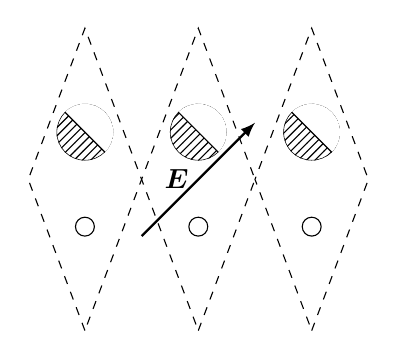
\begin{tikzpicture}[baseline,scale=1.2]
				\draw[dashed] (0,-1.6)--(0.6,0)--(0,1.6)--(-0.6,0)--cycle;
				\begin{scope}
					\clip (0,0.5) circle (0.3);
					\draw[pattern=north east lines] (0,0.5) circle (0.3);
					\draw[fill=white] (0.4,0.1)--(0.4,1.5)--(-0.3,0.8)--cycle;
				\end{scope}
				\draw (0,-0.5) circle (0.1);

				\draw[dashed] (1.2,-1.6)--(1.8,0)--(1.2,1.6)--(0.6,0)--cycle;
				\begin{scope}
					\clip (1.2,0.5) circle (0.3);
					\draw[pattern=north east lines] (1.2,0.5) circle (0.3);
					\draw[fill=white] (1.6,0.1)--(2,1.5)--(0.9,0.8)--cycle;
				\end{scope}
				\draw (1.2,-0.5) circle (0.1);

				\draw[dashed] (-1.2,-1.6)--(-1.8,0)--(-1.2,1.6)--(-0.6,0)--cycle;
				\begin{scope}
					\clip (-1.2,0.5) circle (0.3);
					\draw[pattern=north east lines] (-1.2,0.5) circle (0.3);
					\draw[fill=white] (-0.8,0.1)--(-0.8,1.5)--(-1.5,0.8)--cycle;
				\end{scope}
				\draw (-1.2,-0.5) circle (0.1);

				\draw[thick,->,>=latex] (-0.6,-0.6)--(0.6,0.6);
				\node[left] at (0,0) {$\bm{E}$};
			\end{tikzpicture}
			\caption{{\bf CM Model of Polarization}: A sketch of 2D polarized crystal within CM model. External electric fields $\bm{E}$ are applied in the direction as the arrow does, and shaded areas are the deformed charge density of polarizable anions (big circles), while the cations (small circles) are (assume to be) not.}
			\label{fig:Honeycomb}
		\end{figure}
		However, such choice becomes frustrated for delocalized distribution of electrons because integral \eqref{1.1.3} has to truncate at the region where electron density is nonzero. So any other choice of the primitive cell will result in a different value of eletric polarization. To put it more clear, let us take crystalline silicon as an example. \emph{Ab-initio} calculation is performed under psedopotential implementation of density-functional theory in a series of paper of Hybertsen and Louie in \cite{hybertsen1987ab1,hybertsen1987ab2}, as is shown in FIG. \ref{fig:silicon}. Even though the induced charge displays some dipole-like shapes, one CANNOT find a canonical choice of primitive cell.\par
		\begin{figure}[!htp]
			\centering
			\includegraphics[scale=1]{silicon.pdf}
			\caption{{\bf Induced Charge Density in the $(1\bar{1}0)$ Plane}: In part (a) the pseudo valence charge from a self-consistent local density functional calculation for crystalline silicon is plotted in the $[1\bar{1}0]$ plane. In part (b) the induced charge due to a constant applied electric field in the vertical direction. The contour interval is $2$ electrons per unit cell in both panels Negative contours are indicated by dashedlines. The bond chain is indicated schematically. Figure is extracted from \cite{resta2007theory,hybertsen1987ab2}.}
			\label{fig:silicon}
		\end{figure}
		To eliminate this, one may tempt to define the polarization as intergral over the entire sample
		\begin{equation}\label{1.1.4}
			\bm{P}=\dfrac{1}{V_\text{sample}}\int_{\text{sample}}\dd\bm{r}\,\bm{r}\rho(\bm{r}).
		\end{equation}
		But due to periodicity of our lattice, to ensure the convergence of integral\footnote{Otherwise we will encounter a divergent and meaningless summation of alternating series.} in \eqref{1.1.4}, one must assume a macroscopic but \emph{finite} cystal. And this confinement will inevitablly introduce the contribution from boundary, which cannot be easily disentangled from the bulk's, while we are only interested in \emph{bulk} properties\footnote{In fact the debate whether piezoelectricity or ferroelectricity is a bulk or a surface effect lasted in literature until about 1990s \cite{resta2007theory,tagantsev1991electric}. Nowadays we know that they are both bulk properties \cite{kallin1984surface}.}.\par %On the other hand, most contribution from the deformation of bulk induced charge distribution (like FIG. \ref{fig:silicon}) will be cancelled out  Then Then both bulk contribution and surface contribution will  from 
		Therefore, though counterintuitive, the only conclusion we can draw is that, \textbf{\color{red}a periodic electronic charge distribution in a polarized crystalline solid cannot, even in principle, be used to construct a meaningful definition of \emph{bulk} polarization}.
	
	\subsection{Experimental Aspects}
		One may be disturbing for the conclusion we've drown above. Because bulk properties is natural to be determined by bulk quantanties. But if you stand on the experiemental point of view, all counterintuitive parts seem to become acceptable.\par
		In fact, no matter what kind of polarization we are interested in, in experiments certainly no one relies on the microscopic dipoles for one cell (even if we can and even we successfully obtained, this quantity is still microscopic, rather than macroscopic). Instead, ditto for the spirits of linear-response theory and transport measurement, \textbf{we always put the entire macroscopic sample in a close circuit, imposing some stimulus like external electric field, pressure, or temperature gradient, and then read the macroscopic response $\bm{j}(\bm{r},t)$ from Ampere meter}. Thus what we are measuring is actually the \emph{change} of polarization $\Delta\bm{P}$ under stimulus, given by
		\begin{equation}\label{1.1.5}
			\Delta\bm{P}=\int\dd t\,\dfrac{1}{V_{\text{cell}}}\int_{\text{cell}}\dd\bm{r}\,\bm{j}(\bm{r},t).
		\end{equation}
		Equation \eqref{1.1.5} compares the difference of electric polarization at time $t=0$ and $t=T$. We can safely generalize it to any other \emph{adiabatic evolution} parameterized by $\lambda$ going from $\lambda=0$ to $\lambda=1$ (after re-parameterization)
		\begin{equation}\label{1.1.6}
			\Delta\bm{P}=\int_0^1\dd \lambda\,\dfrac{1}{V_{\text{cell}}}\int_{\text{cell}}\dd\bm{r}\,\bm{j}(\bm{r},\lambda).
		\end{equation}
		Despite the elaborate argument we've shown above, equation \eqref{1.1.5} or \eqref{1.1.6} can also be derived from the microscopic definition of polarization (up to some divergence-free part, which is given by \emph{magnetization}. For a in-depth discussion, see \cite{xiao2010berry,ortiz1994macroscopic} and \cite{hirst1997microscopic})
		\begin{equation*}
			\nabla\cdot\bm{P}(\bm{r})=-\rho(\bm{r})
		\end{equation*}
		and the continuity relation of charge current
		\begin{equation*}
			\dfrac{\partial \rho(\bm{r})}{\partial t}+\nabla\cdot\bm{j}=0.
		\end{equation*}
		\indent Equation \eqref{1.1.6} is indeed a perfect definition because first it avoid the discussion on the bulk charge distribtion so there is no longer problems in canonically selecting primitive cells. Second the boundary contribution polarization is also substracted from the difference. Lastly we do use macroscopic current to define the macroscopic polarization so there is no hierarchy conflict on the philosophy of emergentism in CMP.\par
		
\section{Berry Phase for Bulk Polarization}
	In this section, we will re-written \eqref{1.1.6} by Berry phases with the many-body argument of Niu, Thouless, and Wu \cite{Niu1985quantized} without involvement of non-interacting bloch wave function (TKNN theory) like Resta or Vanderbilt's original paper \cite{king1993theory,resta2007theory} does. Similar discussion can also be found from \cite{ortiz1994macroscopic} or recent paper of Watanabe and Oshikawa \cite{Watanabe2018inequivalent}.
%	\subsection{Review of Thouless Pump}
		Ortiz and Martin first constructed the many-body formulation of bulk polarization in \cite{ortiz1994macroscopic}. Here we try to generalize their work, release the confinement of dimensionality to (d+1)D and focus on the hypercube sample of the volume $V=L_1\times\cdots L_d$.\par
		Suppose eletrons in the bulk insulator subject to a general two-body interaction $V(|\bm{r}_i-\bm{r}_j|)$ from Coulomb scattering, impurity scattering etc., then \emph{many-body} Hamiltonian takes the form of
		\begin{equation}\label{2.1.1}
			H(\lambda)=-\sum_i\dfrac{\hbar^2}{2m_i}\nabla_i^2+\sum_i U(\bm{r}_i,\lambda)+\dfrac{1}{2}\sum_{i\neq j}V(|\bm{r}_i-\bm{r}_j|),
		\end{equation}
		where adiabatic single-body potential $U(\bm{r}_i,\lambda)$ is included as well.\par
		Continuously deforming our setup of close circuit such that multiple faces of our hypercube will connects with others. Similar to \cite{Niu1985quantized}, under so-called magnetic translation \cite{zak1964magnetic} (which is a \emph{large} gauge transformation) our \emph{many-body} wave function allows a particle-indice-indepedent phase shift \cite{Fradkin2013Field}
		\begin{equation}\label{2.1.2}
			\mathscr{T}_i(L_\mu,\hat{x}_\mu)\psi(\bm{r}_i,\lambda)=e^{i \alpha_\mu L_\mu}\psi(\bm{r}_i,\lambda)
		\end{equation}
		because of the total antisymmetry of many-body wave function. Each group of $\{\alpha_\mu\}$ determines one kind of twisted boundary condition of our system.\par
		Eigen problem of $\{\psi(\bm{r}_i,\lambda),H(\lambda)\}$ is equivalent to those differing by just a many-body unitary transformation $\{\phi(\bm{r}_i,\bm{\alpha},\lambda),\widetilde{H}(\bm{\alpha},\lambda)\}$, where
		\begin{equation*}
			\phi(\bm{r}_i,\bm{\alpha},\lambda)\equiv U\psi(\bm{r}_i,\lambda)=\left(\prod_\mu e^{-i \alpha_\mu(x_1+\cdots+x_N)}\right)\psi(\bm{r}_i,\lambda),
		\end{equation*}
		and
		\begin{equation}\label{2.1.3}
			\widetilde{H} (\bm{\alpha},\lambda)\equiv U H(\lambda)U^\dagger =-\sum_i\dfrac{1}{2m_i}\left[\sum_\mu\left(-i\hbar \partial_{i\mu}+i \alpha_\mu\right)^2\right]+\sum_i U(\bm{r}_i,\lambda)+\dfrac{1}{2}\sum_{i\neq j}V(|\bm{r}_i-\bm{r}_j|).
		\end{equation}
		Kinetic part of \eqref{2.1.3} is a reminiscent of the minimal coupling of electromagnetic field. So mathematically $\bm{\alpha}$ can be interpreted as factitious magnetic vector potential $\bm{A}\propto\bm{\alpha}$. Thus for specific boundary condition $\{a_\mu\}$, by definition the current density operator is
		\begin{equation}\label{2.1.4}
			\hat{j}^\mu_{\bm{\alpha}}\equiv\dfrac{\delta \hat{H}}{\delta A_\mu}=\dfrac{\partial \hat{H}(\alpha,\lambda)}{\partial \alpha_\mu}.
			%\bm{j}(\bm{q})\equiv e\bm{v}=e\dot{\bm{r}}=
		\end{equation}
		Macroscopic current density at ``time'' $\lambda$ is given by the thermal and quantum average of many-body ground states
		\begin{equation*}
			j^\mu_{\bm{\alpha}}(\lambda)\equiv\langle\phi(\bm{r}_i,\bm{\alpha},\lambda)|\hat{j}^\mu_{\bm \alpha}|\phi(\bm{r}_i,\bm{\alpha},\lambda)\rangle,
		\end{equation*}
		then adabatic evalution (parameterized by $\lambda$) theory can be applied, giving \cite{bernevig2013topological,xiao2010berry}
\iffalse
		\begin{equation}\label{2.1.5}
			|\phi(\lambda)\rangle=|\phi_n\rangle-i\hbar\sum_{m\neq n}\dfrac{|\phi_m\rangle\langle\phi_m|\partial_\lambda\phi_n\rangle}{\varepsilon_n- \varepsilon_m}
		\end{equation}
\fi
		\begin{equation}\label{2.1.5}
			j^\mu_{\bm{\alpha}}(\lambda)=\partial_{\alpha_\mu} \varepsilon_{\bm{\alpha}}+\Omega^\mu_{\bm{\alpha},\lambda},
		\end{equation}
		where Berry curvature
		\begin{equation}\label{2.1.6}
			\Omega^\mu_{\bm{\alpha},\lambda}\equiv i\bigg[\partial_\lambda\langle\phi|\partial_{\alpha_\mu}\phi\rangle- \partial_{\alpha_\mu}\langle\phi|\partial_\lambda\phi\rangle\bigg].
		\end{equation}
		\indent Since we are working with bulk insulator, where a finite gap always exists during the adabatic evolution, \textbf{the bulk quantity should be insensitive to the deformation of boundary conditions under thermodynamic limit} \cite{Niu1985quantized,Fradkin2013Field}. Therefore we can average over an esemble of many-body system with different boundary condition $0<\alpha_\mu<2\pi/L_\mu$, obtaining
		\begin{equation}\label{2.1.7}
			j^\mu(\lambda)=\prod_\mu\left(L_\mu\int_0^{2\pi/L_\mu}\dfrac{\dd \alpha_\mu}{2\pi}\right)\,j^\mu_{\bm{\alpha}}(\lambda).
		\end{equation}
		Substituting \eqref{2.1.7} to the modern definition of polarization \eqref{1.1.6}, and re-writting $\theta_\mu\equiv \alpha_\mu/L_\mu$, we finally have
		\begin{equation}\label{2.1.8}
			\Delta P^\mu=\int_0^1\dd\lambda\,\int\dfrac{\dd\bm{\theta}}{(2\pi)^d}\,\Omega_{\bm{\theta},\lambda}^\mu.
		\end{equation}
		Equation \eqref{2.1.8} is now the modern definition of macroscopic electric polarization. And it's validity has already been proved in experiments, like \cite{king1993theory}.
\section{Appendix}
	\subsection{Insensitivity of Boundary Condition for Gapped System}
		In this section, we will proof that
		\begin{Claim}
			The difference for the measured macroscopic current for one \emph{fixed} boundary condition $j^\mu_{\bm{\alpha}}$ and the one under average of boundary condition $j^\mu(\lambda)$ drops like $1/L$ and vanishes at thermodynamic limit.
		\end{Claim}
		\begin{Proof}
			The dependence of the macroscopic current on twisted boundary condition $\{\alpha_\mu\}$ enters through the many-body Hamiltonian. And since there is a non-vanishing gap $\Delta_g$ in our system (as a characteristic length), any small changes in parameters of $\bm{\alpha}$ (whose dimension is $[\mathrm{L}]^{-1}$) must lead to changes on $\widetilde{H}(\bm{\alpha})$ of order $\mathcal{O}(\Delta_g)$. Hence
			\begin{equation*}
				\dfrac{\partial j^\mu(\lambda,\bm{\alpha})}{\partial \alpha_\mu}\equiv\dfrac{1}{L_\mu}\dfrac{\partial j^\mu(\lambda,\bm{\theta})}{\partial \theta_\mu}\propto\dfrac{\Delta_g}{L_\mu}\times\text{constant}
			\end{equation*}
		for asymptotically large systems, which vanishes at thermodynamic limit. 
		\end{Proof}
		Another proof of the insensitivity of boundary condition can also be found in the appendix of \cite{Niu1985quantized}.

\bibliography{hxd}
\bibliographystyle{apsrev} % apsrev is format for PRL of APS
\end{document}